\documentclass[a4paper]{article}

\usepackage[utf8]{inputenc}
\usepackage[T1]{fontenc}
\usepackage{textcomp}
\usepackage[english]{babel}
\usepackage{amsmath, amssymb}


%figure support
\usepackage{import}
\usepackage{xifthen}
\pdfminorversion=7
\usepackage{pdfpages}
\usepackage{transparent}
\newcommand{\incfig}[1]{%
	\def\svgwidth{\columnwidth}
	\import{./figures/}{#1.pdf_tex}
}
\graphicspath{ {./figures/} }
\pdfsuppresswarningpagegroup=1

\begin{document}
	\title{CEN4088.01 Lab 9 Due 11/25/19}
	\author{Brandon Thompson 5517}
	\maketitle

	\begin{figure}[ht!]
		\centering
		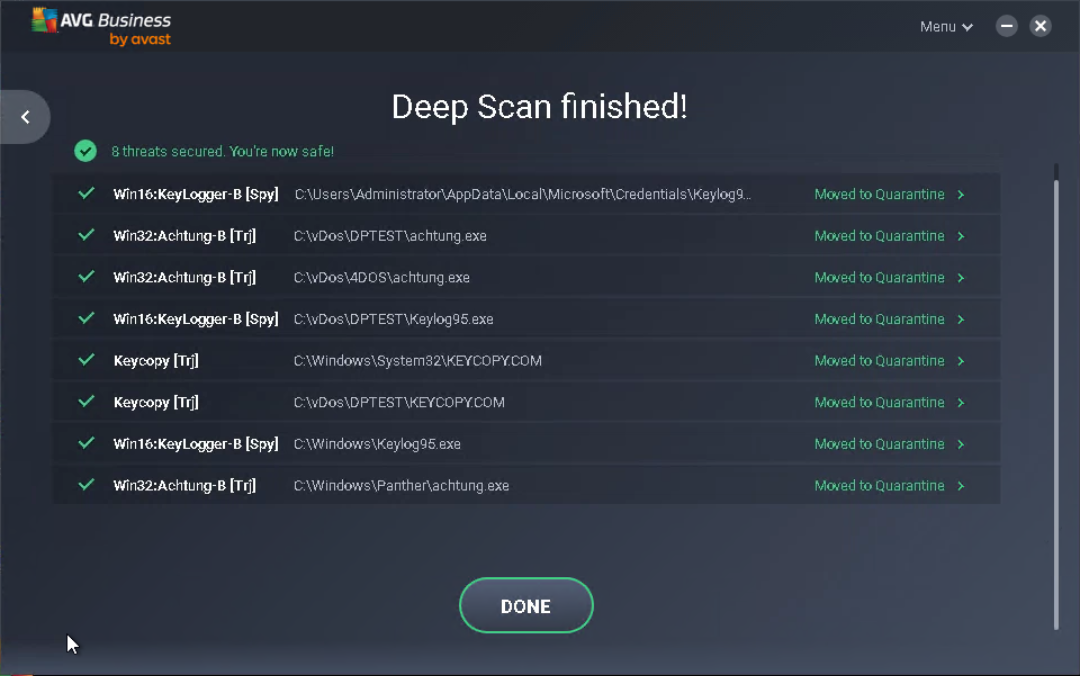
\includegraphics[width=0.8\textwidth]{1_2_7}
		\caption{AVG scan summary of TargetWindows02.}
		\label{fig:1_2_7}
	\end{figure}
	\begin{figure}[ht!]
		\centering
		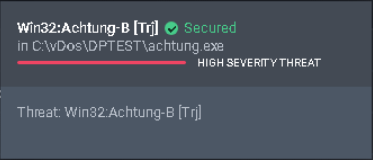
\includegraphics[width=0.8\textwidth]{1_3_2}
		\caption{Details of \texttt{achtung.exe} threat.}
		\label{fig:1_3_2}
	\end{figure}
	The \texttt{achtung.exe} file is associated with a virus called Entangle Worm (W32.Entangle.Worm).
	The entangle worm is a mass-mailing worm that will send itself to all addresses in the
	windows address book and copy itself to the \%System\% and \%temp\% environments. To remove
	the worm, ensure that virus definitions are updated and scan the system with AVG Business.\\
	\begin{figure}[ht!]
		\centering
		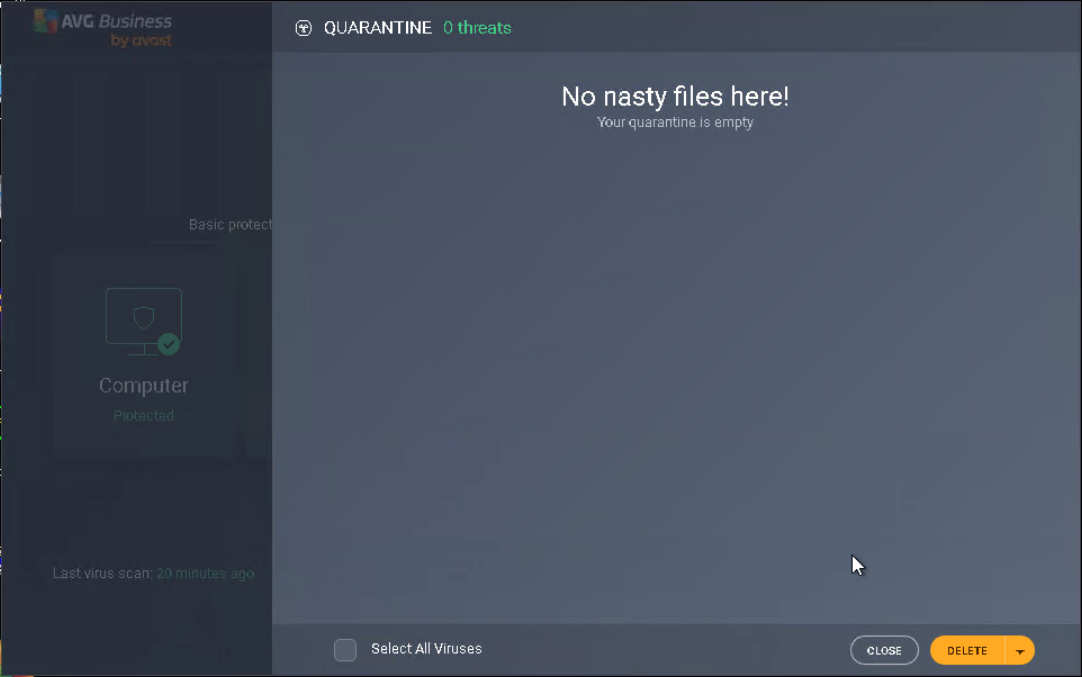
\includegraphics[width=0.8\textwidth]{1_3_10}
		\caption{Empty quarantine area (virus vault).}
		\label{fig:1_3_10}
	\end{figure}

	\section*{Security Incident Report Part 1}
	\textbf{Incident Report \#:} IR-83631\\
	\textbf{Report Date and Time:} 11/21/19 10:00 AM\\
	\textbf{Technician:} Brandon Thompson\\
	\textbf{Site Location:} Virtual machine IP 172.30.0.10 (Windows Server 2016)\\
	\\
	Identification (type and how detected): Part of lab exercise.\\
	\\
	\textbf{Virus scan detected:} Keylogger and Avalanche (\texttt{achtung.exe}).\\
	Triage (impact): Virtual machine 172.30.0.10 only.\\
	\\
	Containment (Steps taken):
	\begin{enumerate}
		\item Disabled wireless on virtual machine.
		\item Ran manual virus detection
	\end{enumerate}
	Investigation (Cause): worm placed on machine for education purposes.\\
	Recovery and Repair (Resolution):\\
	\\
	Used antivirus software to quarantine and eradicate the malware.\\
	Implemented scanning of email for malware and spam.\\
	Lessons Learned (Debriefing and Feedback):\\
	\\
	Antivirus software on systems should be configured to scan all hard drives regularly to
	identify any file system infections and, optionally, to scan other storage media as well.
	Users should also be able to launch a scan manually as needed.\\
	\\
	Users should be educated on protecting themselves from viruses by running only company
	authorized Antivirus software, not opening suspicious e-mail attachments, not responding
	to suspicious or unwanted e-mails.\\
	\\
	\begin{figure}[ht!]
		\centering
		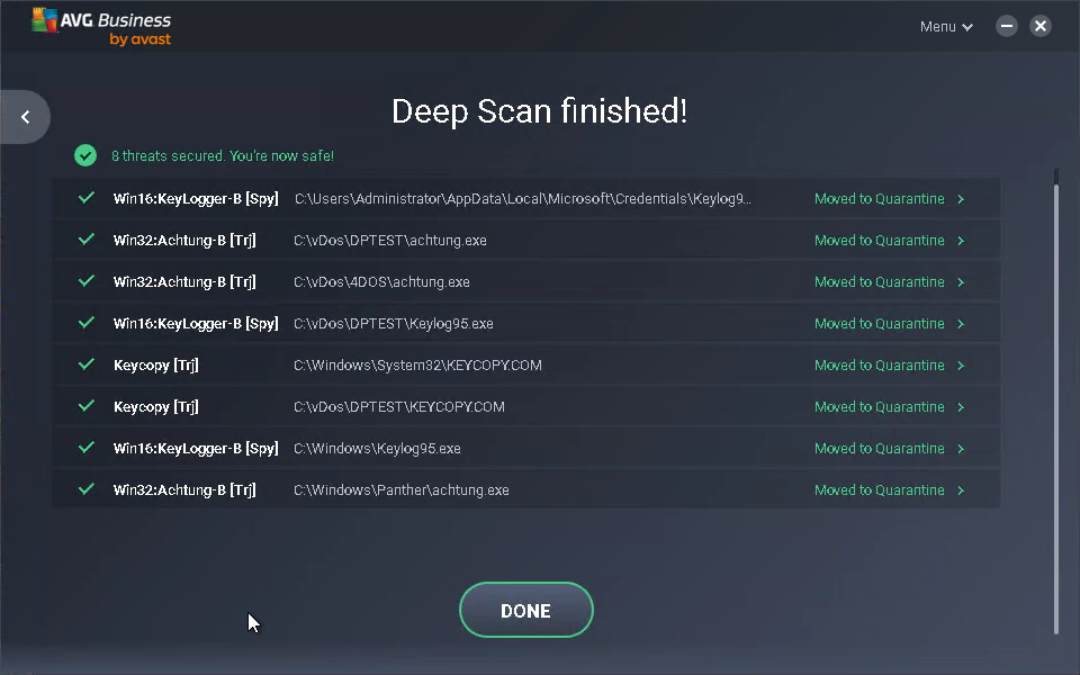
\includegraphics[width=0.8\textwidth]{2_2_8}
		\caption{AVG scan summary of TargetWindows02.}
		\label{fig:2_2_8}
	\end{figure}

	\begin{figure}[ht!]
		\centering
		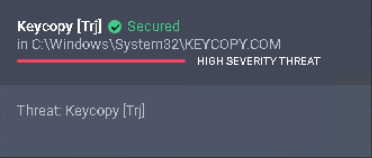
\includegraphics[width=0.8\textwidth]{2_3_2}
		\caption{Details of KEYCOPY.COM}
		\label{fig:2_3_2}
	\end{figure}

	The \texttt{KEYCOPY.COM} file is associated with a keylogger virus that records keystrokes and
	applications to retrieve usernames and passwords to gain access to secure information.
	Keycopy.com gains access to the computer through installing malicious software or files from
	untrusted websites. To remove the keycopy.com virus from the system ensure virus definitions
	are up to date and scan the system with AVG Business.
	
	\begin{figure}[ht!]
		\centering
		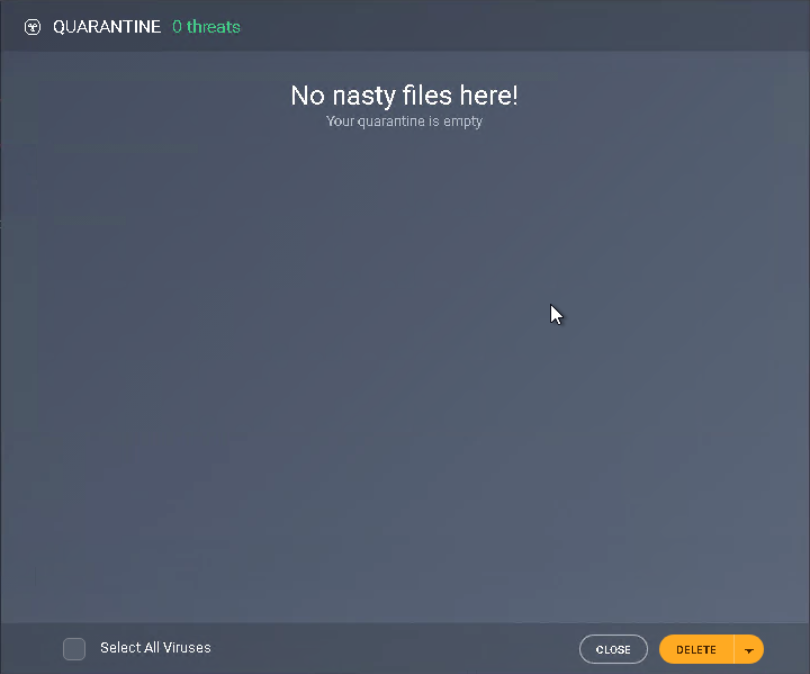
\includegraphics[width=0.8\textwidth]{2_3_9}
		\caption{Empty quarantine area.}
		\label{fig:2_3_9}
	\end{figure}

	\section*{Security Incident Report Part 2}
	\textbf{Incident Report \#:} IR-83632\\
	\textbf{Reported Date and Time:} \today\\
	\textbf{Technician:} Trevor Dash\\
	\textbf{Site Location:} Virtual machine IP 172.30.0.10 (Windows Server 2016)\\
        \\
	Identification (type and how detected): Part of lab exercise.\\
        \\
        \textbf{Virus scan detected:} Keylogger Virus (\texttt{KEYCOPY.COM}).\\
        Triage (impact): Virtual machine 172.30.0.10 only.\\
        \\
        Containment (Steps taken):
        \begin{enumerate}
                \item Disabled wireless on virtual machine.
                \item Ran manual virus detection
	\end{enumerate}
        Investigation (Cause): worm placed on machine for education purposes.\\
        Recovery and Repair (Resolution):\\
        \\
        Used antivirus software to quarantine and eradicate the malware.\\
        Implemented scanning of email for malware and spam.\\
        Lessons Learned (Debriefing and Feedback):\\
        \\
        Antivirus software on systems should be configured to scan all hard drives regularly to
        identify any file system infections and, optionally, to scan other storage media as well.
        Users should also be able to launch a scan manually as needed.\\
        \\
        Users should be educated on protecting themselves from viruses by running only company
        authorized Antivirus software, not opening suspicious e-mail attachments, not responding
        to suspicious or unwanted e-mails.\\
        
\end{document}
